\documentclass[12pt]{ociamthesis}  % default square logo 
%\documentclass[12pt,beltcrest]{ociamthesis} % use old belt crest logo
%\documentclass[12pt,shieldcrest]{ociamthesis} % use older shield crest logo

%load any additional packages
\usepackage{amssymb}
%encoding
%--------------------------------------
\usepackage[T1]{fontenc}
\usepackage[utf8]{inputenc}
%--------------------------------------
 
%Portuguese-specific commands
%--------------------------------------
\usepackage[portuguese]{babel}
\usepackage{natbib}


%Incluir um arquivo em PDF
%--------------------------------------
\usepackage{pdfpages}


%input macros (i.e. write your own macros file called mymacros.tex 
%and uncomment the next line)
%\include{mymacros}

\title{Análise Estrutural da Bacia do Parnaíba através da Função do Receptor e das Curvas de Dispersão calculadas a partir de Terremotos e Ruído Sísmico Ambiental\\        }   %note \\[1ex] is a line break in the title
\author{
Orientando:\\
Diogo Luiz de Oliveira Coelho\\
Orientador:\\
Jordi Julià Casas}   %your name

%\college{}  %your college

%\renewcommand{\submittedtext}{change the default text here if needed}
\degreedate{Natal, Brasil 2017}         %the degree date

%end the preamble and start the document
\begin{document}

%this baselineskip gives sufficient line spacing for an examiner to easily
%markup the thesis with comments
\baselineskip=18pt plus1pt

%set the number of sectioning levels that get number and appear in the contents
\setcounter{secnumdepth}{3}
\setcounter{tocdepth}{3}

\maketitle                  % create a title page from the preamble info
\begin{romanpages}          % start roman page numbering
\addcontentsline{toc}{chapter}{Resumo}
\chapter*{Resumo}

A gênese e evolução de grandes bacias sedimentares no interior de continentes estáveis é um importante problema geológico que não é facilmente compreendido dentro do paradigma da Tectônica de Placas. A bacia do Parnaíba é uma das três grandes bacias sedimentares Paleozóicas na plataforma Sulamericana - junto com as bacias do Paraná e Amazonas. A bacia é comumente descrita como uma grande bacia cratônica do tipo sag com uma forma semi-circular e um depocentro que chega a profundidades de 3.5 km. Já o mecanismo físico que atuou na sua subsidência e evolução, em contrapartida, é muito controverso. Vários mecanismos de formação foram propostos nessa bacia, mas o conhecimento sobre a arquitetura crustal e mantélica abaixo da bacia do Parnaíba ainda é muito pequeno. Devido a isso, nós propomos investigar a arquitetura crustal abaixo da bacia do Parnaíba através da análise das Funções do Receptor e da tomografia de ruído ambiental, para imagear estruturas profundas e rasas, respectivamente. Na primeira parte do nosso trabalho, nós apresentamos estimativas pontuais de espessura crustal e razão Vp/Vs em 9 estações numa transecta NW-SE na parte central da bacia, junto com perfis de velocidade de onda S obtidos na inversão conjunta entre funções do receptor e velocidades de ondas de superfície. Essa análise revela a crosta como sendo espessa com 44-45 km em média no depocentro e um afinamento progressivo de 39-41 km em direção às bordas, enquanto que a razão Vp/Vs varia entre  1.70 e 1.78 ao longo da transecta, com grandes valores próximo ao depocentro. Os perfis de velocidade confirmam essa variação da espessura crustal e revelam uma crosta inferior de 18-22 km de profundidade com velocidades variando de 3.7 a 3.8 km/s, mas que podem chegar a 4.0-4.2 km/s perto do depocentro. Nossos resultados favorecem modelos de formação de bacia que possuem um estiramento crustal mínimo e são compatíveis com dobramentos flexurais devido a uma carga em profundidade. No entanto, não se observa a existência de um grande corpo intrusivo na crosta inferior. Arguimos que processos convectivos profundos na astenosfera podem prover tal mecanismo de carga. A segunda parte do nosso trabalho consistirá no imageamento da zona de transição do manto com funções de receptor para ver qual o comportamento da astenosfera abaixo da bacia. Além disso, utilizaremos o ruído ambiental para analisar as estruturas crustais rasas, principalmente para entender o efeito do lineamento Transbrasiliano na formação da bacia.            % include the resumo
\addcontentsline{toc}{chapter}{Abstract}
\chapter*{Abstract}
The genesis and evolution of large basins in the stable interiors of continents is an important geological problem that is not easily understood within the Plate Tectonics paradigm. The Parnaíba basin is one of three large Paleozoic basins in stable South America - together with the Paraná and Amazon basin. The basin is commonly described as a large, sag-type cratonic basin, with a roughly circular shape and a depocenter reaching up to 3.5 km depth. The physical mechanism behind its subsidence and evolution, on the other hand, is more controversial. A number of basin-forming mechanisms have been proposed for this basin, but the knowledge about the deep architecture of this cratonic basin is very little yet. Owing to that, we propose to investigate the crustal and mantle architecture beneath of the Parnaíba basin by analyzing P-wave receiver functions and ambient noise tomography, to image deep and shallow structures, respectively. In the first part of our work, we present point estimates of crustal thickness and Vp/Vs ratio at 9 broadband stations in a 600 km-long transect crossing the central portion of the basin, along with detailed S-wave velocity-depth profiles obtained from the joint inversion of P-wave receiver functions and surface-wave dispersion velocities. This analysis reveals the crust could be as thick as 44-45 km around the basin’s depocenter and that it progressively thins to 39-41 km towards the edges, while bulk Vp/Vs ratios are in the 1.70-1.78 range along the transect, with larger values around the depocenter. The velocity-depth profiles confirm crustal thickness variations and reveal a lower crustal layer below 18-22 km depth, with S-velocities in the 3.7-3.8 km/s range that locally raise to 4.0-4.2 km/s near the depocenter. Our findings favor models invoking minimal stretching of the basin’s underlying crust and are found compatible with flexural bending by a deep load. However, the existence of a thick intrusive body pervading the lower crust is not supported by our results. We argue that deep convective processes in the asthenosphere might provide an alternative loading mechanism. The second part of our work will consists of imaging the transition zone of the mantle with P-wave receiver functions to see how is the behavior of the asthenosphere beneath the basin. Furthermore, to use the ambient noise to analyse the shallow crustal structures of the basin, mainly to understand the Transbrasiliano lineament effect in the basin evolution.
          % include the abstract

\tableofcontents            % generate and include a table of contents
%\listoffigures              % generate and include a list of figures
%\listoftables               % generate and include a list of tables
        
\end{romanpages}            % end roman page numbering

%now include the files of latex for each of the chapters etc

\chapter{Introdução}


\section{Escopo}

Este exame de qualificação está estruturado em seis partes. A primeira parte
trata da apresentação do tema, com objetivos, justificativas e as estapas propostas no projeto de doutorado que foram concluídas, ou não. A segunda parte compõe um breve resumo sobre o paradigma da formação e evolução de bacias intracratônicas. A terceira parte apresenta a síntese do arcabouço geológico da Bacia do Parnaíba, mostrando um sumário sobre o preenchimento sedimentar, magmatismo e tectônica proposta em trabalhos anteriores. A quarta parte apresenta um artigo intitulado: \textit{"Deep crustal architecture of the Parnaíba basin of NE Brazil from receiver function analysis: Implications for basin subsidence"} que foi submetido para a The Geological Society Special Publications em março deste ano. A quinta e sexta partes propõem temas a serem estudados nos próximos semestre, como descontinuidades mantélicas de 410 km e 660 km através das funções do receptor e a tomografia de ruído sísmico ambiental, respectivamente.

\section{Objetivos}

Esta tese de doutorado tem por objetivo principal a caracterização estrutural, tanto crustal quanto mantélica, da Bacia do Parnaíba para buscar informações nesse arcabouço estrutural sobre os processos de formação e evolução na bacia. Com essa finalidade, foram elaborados objetivos secundários:

\begin{enumerate}
\item Determinação das estruturas crustais profundas na bacia atráves das estimativas pontuais de espessura crustal e razão Vp/Vs junto com perfis de velocidade de onda S obtidos na inversão conjunta entre funções do receptor e velocidades de ondas de superfície;

\item Imageamento das descontinuidades mantélicas de 410 km e 660 km, limites inferior e superior da Zona de Transição, para entender o papel da temperatura na evolução geológica da bacia;

\item Imagear o lineamento Transbrasiliano dentro da bacia atravéns da tomografia de ruído sísmico ambiental para entender o papel dessa mega-estrutura na formação e evolução da bacia;

\item Gerar subsídios para a proposição de um modelo de formação e evolução da Bacia do Parnaíba.

\end{enumerate}
\section{Justificativa}

A Bacia do Parnaíba, mesmo com um grande número de trabalhos realizados recentemente, ainda carece de muita informação sobre seu arcabouço estrutural crustal e mantélico. Esta bacia é tomada como paradigma para compreender o porquê de grandes áreas no interior de continentes, consideradas estáveis, em certos momentos de sua história passam por longos estágios de subsidência, ao longo dos quais são acumulados pacotes de rochas sedimentares com vários quilômetros de espessura associadas a manifestações vulcânicas episódicas. A maior parte do conhecimento sobre esta bacia é restrito a uma escala continental, como os estudos de \cite{feng_group_velocity_2004}, \cite{feng_upper_2007}, \cite{lloyd_moho_2010},\cite{van_der_meijde_gravity_2013},\cite{assumpcao_crustal_2013},\cite{assumpcao_models_2013},\cite{goutorbe_rayleigh_2015} e \cite{uieda_fast_2017}, e recentemente trabalhos regionais como os de \cite{de_castro_crustal_2014},\cite{daly_brasiliano_2014}, \cite{de_castro_geophysical_2016} e \cite{tozer_crustal_2017}. 

O presente trabalho encontra-se vinculado ao \textit{Parnaíba Basin Analysis Project}, uma parceria entre a BP Energy do Brasil  e várias universidades no Brasil e no Reino Unido, e tem com o objetivo melhorar o conhecimento sobre a origem e evolução dessa grande bacia cratônica no Norte-Nordeste do Brasil. Tal bacia é considerada uma fronteira exploratória, devido a descoberta de campos de gás natural durante a última década. Devido à sua grande dimensão, a maior parte do substrato sobre o qual a Bacia do Parnaíba se desenvolveu encontra-se encoberta, de forma que as informações disponíveis advêm majoritariamente de forma indireta. A análise conjunta de dados sismológicos, oriundos de sismos e de ruído ambiental, possibilita uma melhor resolução na observação de estruturas profundas e rasas no interior da bacia.

\section{Cronograma de Execução}

Após realizar as disciplinas propostas no projeto de Doutorado e ter um coeficiente de rendimento médio superior a 4, as únicas componentes curriculares obrigatórias pendentes são: Seminário de Pesquisa II, Exame de Qualificação, Exame de Proficiência em outra língua estrangueira diferente de inglês e Tese de Doutorado. Dos quais o Seminário de Pesquisa II e Exame de Qualificação eu já me encontro matriculado e devo cumprir no fim desse semestre. Restando apenas um exame de proficiência que devo cumprir no começo do próximo semestre e, por fim, a Defesa da Tese no final de 2018. 

\begin{figure}[!ht]
\begin{center}
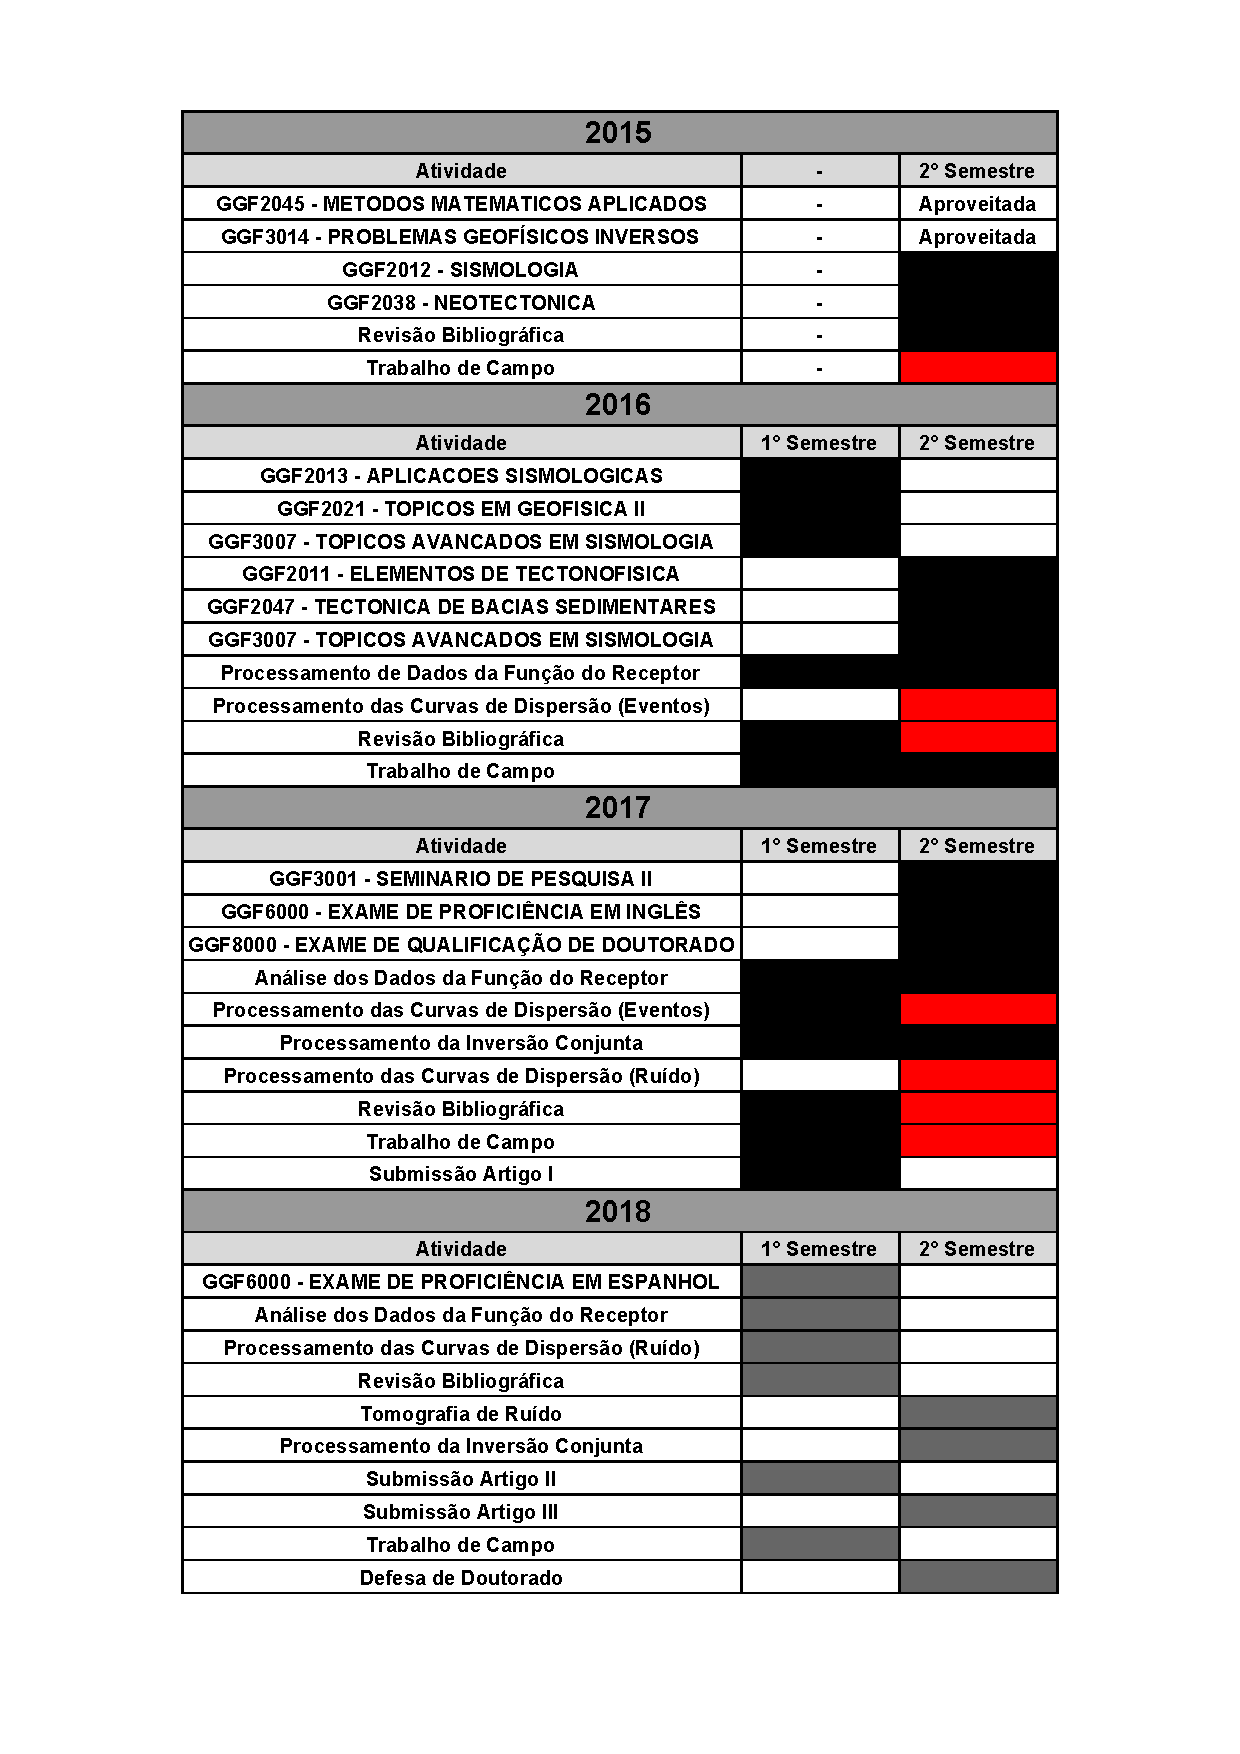
\includegraphics[width=1\textwidth]{Fig/cronograma.pdf}
\caption{Cronograma proposto no projeto de Doutorado. Preto - Etapas concluídas, Vermelho - estapas não concluídas na época prosposta, Cinza - Etapas futuras}
\label{mapa_sta_mantle}
\end{center}
\end{figure}
\chapter{Modelos de Formação de Bacias Intracratônicas}

\cite{allen_cratonic_2012} utiliza o termo bacia cratônica para com as bacias localizadas distantes de margens continentais convergentes e localizados numa variedade de substratos crustais, independentemente de serem escudos cristalinos, cinturões de dobramentos antigos e riftes complexos. Segundo \cite{armitage_subsidence_2010}, pode-se considerar que o interior dos continentes não sofre com a convecção do manto subjacente e com a tectônica de placas operante. No entanto, grandes regiões da litosfera continental estável tem experimentado ciclos de subsidência prolongada e de soerguimento, gerando grandes bacias. A principal feição das bacias cratônicas é o seu período de subsidência prolongada, o qual se iniciaria durante períodos de dispersão continental e podem continuar através de ciclos de fechamento de oceanos e colisão continental. Elas estão situadas no interior de margens passivas, mas são comumente conectadas ao oceano por riftes falhados que estão orientados em alto ângulo com a margem da placa, possíveis braços abortados de junções tríplices.

\cite{allen_cratonic_2012} mostra que apesar das individualidades de cada bacia, existem várias feições estruturais que podem ser comuns entre as bacias cratônicas, como: (1) a área da superfície ao redor da isópaca zero do preenchimento sedimentar é comumente circular ou elíptica; (2) em corte essas bacias possuem formato de pires, mostrando uma falta de falhas sin-tectônicas e uma espessura sedimentar menor que 5 km de profundidade; (3) a duração da subsidência é muito longa, por volta de centenas de milhões de anos, e as curvas de subsidência tectônica oriundas do backstripping apresentam uma tendência sublinear a um exponencial negativo suave. Essa longevidade da subsidência geralmente compreende várias fases de deposição da bacia separadas por inconformidades, gerando megasequências sobrepostas, que são produtos das mudanças na tectônica operante na época de deposição; (4) a estratigrafia é predominantemente de ambiente terrestre a marinho-raso, indicando que a sedimentação acompanhou o ritmo da subsidência tectônica. As bacias cratônicas em baixas paleolatitudes são geralmente dominadas por sedimentos quimiogênicos, mostrando que o suprimento de sedimento em partículas era modesto, e que altos topográficos estavam ausentes em torno das margens das bacias nesses locais; (5) bacias cratônicas são comumente espaçadas regularmente com seus centros localizados cerca de $10^{3}$ km de distância das bordas; (6) algumas bacias cratônicas estão associadas com o magmatismos amplamente difundidos, como a erupção de grandes volumes de basaltos. No entanto, as ligações entre o vulcanismo e o desenvolvimento da bacia ainda não são claras.  

Existem inúmeras tentativas de explicar a origem e o desenvolvimento de grandes bacias  sedimentares intracratônicas extensas e longevas, como pode ser visto nos trabalhos de \cite{hartley_interior_1994,kaminski_lithosphere_2000,armitage_subsidence_2010,mkenzie_speculations_2016}. O preenchimento sedimentar desse tipo de bacia raramente mostra-se falhado, sugerindo que deformação frágil raramente acompanha a subsiedência. \cite{hartley_interior_1994} propõem que a baixa a moderada maturidade dos indicadores termais nos sedimentos da bacia não está associada com as principais distorções termais da litosfera. Existiram dois períodos na história da Terra quando a iniciação de bacias cratônicas tem sido importantes, ambos relacionados com a quebra de assembléias supercontinentais. As bacias cratônicas antigas das quais se possuem mais dados são as pertencentes ao Craton norte-americano, que são associadas com a quebra do continente Laurência no começo do Paleozóico, como observado no trabalho de \cite{kaminski_lithosphere_2000}. 

\cite{hartley_interior_1994} e \cite{allen_cratonic_2012} enumeram as hipóteses propostas na literatura para explicar a criação e evolução das bacias intracratônicas, como (1) estiramento litosférico seguido de uma contração termal,  (2) mudanças de fase crustais e mantélicas,  metamorfismo e intrusão, (3) tensão planar ou rejuvenescimento tectônico, (4) instabilidades convectivas no manto, e (5) erosão subaérea de estruturas soerguidas. No entanto, uma melhor compreensão dos mecanismos de formação das bacias cratônicas é dificultada pela falta de conhecimento de algumas condições pretéritas das bacias. Além disso, o momento atual é um dispersão continental em vez de uma de ruptura supercontinental, como resultado, as bacias cratônicas podem ser características menos comuns da superfície da Terra hoje, quando comparadas a certos momentos no passado geológico, logo o observação de todos os fatores na formação e evolução deste tipo específico de bacia sedimentar é dificultada.





\chapter{Arcabouço Geológico da Bacia do Parnaíba}

A Bacia do Parnaíba é uma das grandes bacias intracratônicas paleozoicas do Brasil, junto com as bacias do Paraná, Solimões e Amazonas. Sua área extende-se por 600 mil $km^{2}$ na porção Norte e Nordeste do Brasil, englobando os estados do Piauí, Maranhão, Tocantins, Pará, Ceará e Bahia. Em seu depocentro, é possível observar espessuras próximas de 3.500 metros de profundidade \citep{goes_feijo_1994,vaz_bacia_2007}. Regionalmente, a Bacia do Parnaíba é bordejada por blocos cratônicos e por faixas de dobramentos brasilianas \citep{cordani_bacia_2009,de_castro_crustal_2014}. Ao norte a bacia é limitada pelas bacias sedimentares da Margem Equatorial, o Cráton São Luís e pela Faixa Gurupi. Já a oeste, pela Faixa Araguaia e pelo Cráton Amazônico. Ao leste e sul, encontra-se o Cráton São Francisco e a Província Borborema, como pode ser visto na Figura \ref{mapa_geologico}.

\begin{figure}[!ht]
\begin{center}
\includegraphics[width=1\textwidth]{Fig/mapa_geologico_eras.pdf}
\caption{Mapa geológico da Bacia do Parnaíba.}
\label{mapa_geologico}
\end{center}
\end{figure}

\section{Preenchimento Sedimentar}

\cite{goes_formacao_1995} aponta a dificuldade da compreensão do histórico deposicional da bacia junto com a compartimentação tectônica pré, sin e pós-ruptura do Macrocontinente Gondwana, devido a um preenchimento sedimentar com gênese, estilo tectônico e idade distinta. Com a dificuldade de relacionar todo esse registro sedimentar a uma única unidade geotectônica, sugeriu-se uma série de sub-bacias compondo uma grande provincia sedimentar, chamada Província Sedimentar do Meio-Norte. Já os trabalhos de \cite{vaz_bacia_2007,daly_brasiliano_2014,de_castro_geophysical_2016,tozer_crustal_2017} entendem que a Bacia do Parnaíba tem uma história deposicional marcada por 5 sequências tectôno-sedimentar primárias e dois pulsos magmáticos seperados por descontinuidades geológicas regionais. O preenchimento sedimentar da bacia é caracterizado pelas sequências: Riachão, Jaibaras, Parnaíba, Mearim e Grajaú. \cite{vaz_bacia_2007} mostra que as sequências Riachão e Jaibaras formam um embasamento sedimentar da Bacia do Parnaíba. Porém existe uma diversidade de interpretações sobre a formação e idades dessas sequências sedimentar, principalmente para a sequências Richão, como é visto nos trabalhos de \cite{de_castro_geophysical_2016} e \cite{tozer_crustal_2017}. As sequências inicias são interpretadas como sedimentos pretéritos oriundos de eventos de riftiamentos neoproterozóicos e cambro-ordovicianos, como mostra \cite{de_oliveira_jaibaras_2003} e \cite{de_castro_crustal_2014}. A tectônica e idade dessas sequências ainda encontra-se em discussão nas pesquisas atuais, fato que não iremos abordar neste trabalho, pois não faz parte do escopo, mas pode ser observado nos trabalhos de \cite{de_castro_crustal_2014,daly_brasiliano_2014,de_castro_geophysical_2016,tozer_crustal_2017}.

A tectono-sequência Parnaíba é relacionada a uma bacia cratônica do tipo sinéclise, denominada por \cite{goes_formacao_1995} como a Bacia do Parnaíba, propriamente dita. Essa tectono-sequência tem idade entre o Ordoviciano Tardio até o incío do Triássico e consiste de três megasequências separadas por inconformidades regionais, como pode ser visto em \cite{daly_brasiliano_2014}. Estes depósitos são caracterizados por camadas apresentando grande continuidade e espessuras regulares que se afinam progressivamente em direção às bordas da bacia, um comportamento característico do estilo de bacia do tipo sag. Os tipos de sedimentos associados a essa fase são marinhos rasos, fluvio-lacustre e siliciclásticos terrestres. 

\cite{vaz_bacia_2007} mostra que a tectono-sequência Mearim, ou Jurássica, é composta apenas pela Formação Pastos Bons, que corresponde a depósitos lacustrinos com contribuição fluvial, em clima semi-árido a árido. A sequência é balizada na base e no topo por episódios magmáticos e é restrita apenas ao centro da bacia \citep{tozer_crustal_2017}. Já a tectono-sequência Grajaú (Cretácea) é caracterizada por depósitos marinhos rasos, lacustres e flúvio-deltaicos, cuja deposição seria reflexo da abertura do Oceano Atlântico \citep{vaz_bacia_2007}. Em afloramento, essa seqüência ocorre principalmente na porção noroeste-norte da bacia e sobrepõe-se discordantemente sobre as rochas das seqüências mais antigas. É importante frisar que o depocentro se deslocou durante a fase deposicional da bacia, com uma forte tendência para oeste, como mostra \cite{tozer_crustal_2017} através de dados de backstripping. 

\section{Magmatismo}

A intensa atividade ígnea em que foram palcos as bacias do Parnaíba, Paraná, Amazonas e Solimões teve início com a abertura da Margem Equatorial durante a separação entre os continentes sul-americano e africano. Segundo \cite{vaz_bacia_2007} a Bacia do Parnaíba acomodou rochas ígneas intrusivas, diques e soleiras, e extrusivas de composição básica, as quais foram divididas em duas unidades: Formação Mosquito e Formação Sardinha. Essas formações são correlacionadas às rochas originadas a partir do rifteamento do supercontinente Pangea e da abertura do Oceano Atlântico, respectivamente. As idades isotópicas calculadas por \cite{merle_40ar_39ar_2011} apontam que a Formação Mosquito pertence à Província Magmática do Atlântico Central, já a formação Sardinha seria associada à Província Magmática Paraná-Etendeka.

Eventos precursores à desagregação do Gondwana Oeste propiciaram o abatimento da região central da bacia, com a formação de um sistema de riftes interiores, preenchidos pelos sedimentos das formações Pastos Bons e Corda associados ao alojamento das rochas básicas das formações Mosquito e Sardinha. A implantação desses riftes ocorreu, principalmente, sobre área da Estrutura de Xambioá, como mostra \cite{mocitaiba_cartografia_2017}. As estruturas grabenformes geradas permitiram o alojamento desses eventos ígneos mesozoicos. Em subsuperfície, os diques da Formação Sardinha e as soleiras da Formação Mosquito estão presentes em maior quantidade na tectono-sequência paleozoicas \citep{vaz_bacia_2007}.

\section{Tectônica}

A bacia do Parnaíba é circundada por inúmeras massas cratônicas arqueanas e por cinturões de dobramentos proterozoicos, como pode ser visto na Figura \ref{mapa_geologico}. Dois desses principais blocos formaram duas grandes massas continentais (São Franciso-Congo e São Luís-West Africa) que existiram antes da abertura do oceano Atlântico no mesozoico, e estavam envolvendo o bloco da Parnaíba, provável massa cratônica coberta pela bacia homônima. A existência desse bloco ocultado pela cobertura sedimentar foi postulada por inúmeras trabalhos nos ramos da geofísica, petrofísica, tectônica e geocronologia \citep{de_brito_neves_influence_1984, cordani_bacia_2009,fuck_rodinia_2008,de_castro_crustal_2014}. Análises de dados magnéticos e gravimétricos recentemente subdividiram esse bloco Parnaíba em pequenos fragmentos, denominados Parnaíba Norte, Parnaíba Sul e Teresina. Estes caracterizados pelas mudanças marcantes nas propriedades magnéticas e pelas variações de até 3.5 km na espessura crustal \citep{de_castro_crustal_2014}. 

No passado, estudos geofísicos da Bacia do Parnaíba delinearam uma grande quantidade de estruturas grabenformes abaixo da cobertura sedimentar, como mostra \cite{de_brito_neves_influence_1984,cordani_bacia_2009}. Essas estruturas interpretadas foram utilizadas como suporte para modelos de subsidência termo-mecânicos, como o clássico modelo de \cite{mckenzie_remarks_1978}. Um refinamento mais recente deste conjunto de modelos foi proposto por \cite{de_castro_crustal_2014}, pela análise de anomalias gravimétricas e magnéticas. Os autores identificaram dois conjuntos de trends lineares no embasamento, o qual foram interpretados como dois estágios de riftiamento, um relacionado ao fim da orogenia Brasiliana e o outro precedendo a fase deposicional principal da bacia no Cambro-Ordoviciano. 
Em um grande perfil de reflexão sísmica profunda \cite{daly_brasiliano_2014} não encontrou evidência de uma fase de riftiamento neoproterozóica postulada previamente, e notou uma inconformidade subplanar cortando todos os blocos crustais interpretados no perfil, Borborema, Parnaíba e Amazônico. Segundo os autores, os limites principais e as estruturas do embasamento não teriam uma grande influência na formação da bacia e propõem que uma subsidência termal se tornaria um provável mecanismo para a formação e evolução da bacia do Parnaíba.

A viabilidade de um modelo de riftiamento para a bacia foi investigada exaustivamente por \cite{tozer_crustal_2017} através dos estudos das anomalias Bougher desenvolvidas em cima do mesmo perfil sísmico de \cite{daly_brasiliano_2014}, backstripping dos dados de poços disponíveis e da modelagem sísmica de uma rede densa de receptores no centro da transecta. O estudo demonstrou que o modelo de riftiamento não é capaz de explicar as estruturas crustais inferidas, assim como a história de subsidência dessa bacia. Devido a grande quantidade de intrusões magmáticas na bacia, os autores postularam existência de uma grande corpo máfico de 12-20 km de espessura na crosta inferior que serviria como um carga que causaria uma subsidência flexural. Através da relaxão do esforço viscoelástico essa carga poderia explicar a longa história de subsidência observada nos registros de poços. No entanto, os autores não restringem os limites dessa carga em profundidade e ainda não existem evidências geológicas de um magmatismo extensivo no início da bacia, prova cabal para poder afirmar esse corpo magmático na crosta inferior.
\chapter{Artigo: Deep crustal architecture of the Parnaíba basin of NE Brazil from receiver function
analysis: Implications for basin subsidence}

O artigo intitulado: \textit{"Deep crustal architecture of the Parnaíba basin of NE Brazil from receiver function analysis: Implications for basin subsidence"} foi submetido para a The Geological Society Special Publications e passa pela segunda revisão no momento. Este artigo corresponde a estimativas pontuais de espessura crustal e razão Vp/Vs em 9 estações numa transecta NW-SE na parte central da bacia, junto com perfis de velocidade de onda S obtidos na inversão conjunta entre funções do receptor e velocidades de ondas de superfície. 

\includepdf[pages=-]{GSL_paper.pdf}
\chapter{Artigo: Receiver function imaging of mantle transition zone discontinuities beneath Parnaíba Basin}

Essa seção corresponde a segunda etapa do projeto, a qual consiste em observar as descontinuidades mantélicas de 410 km e 660 km, limites inferior e superior da Zona de Transição, abaixo da bacia do Parnaíba com as funções do receptor. Os limites da Zona de Transição e sua espessura são dependentes da temperatura, logo quando estão associados a anomalias termais essas descontinuidades de 410 km e 660 km devem ser imageadas a uma profundidade diferente da convencionada pelos modelos de velocidade globais. Para isso, apresentaremos empilhamentos e a migração em profundidade das funções do receptor para 9 estações na transecta NW-SE na parte central da bacia, como pode ser visto na Figura \ref{mapa_sta_mantle}.

\begin{figure}[!ht]
\begin{center}
\includegraphics[width=1\textwidth]{Fig/mapa_topografico_estacoes.pdf}
\caption{Mapa com as estações da rede da BP na transecta NE-SW na Bacia do Parnaíba.}
\label{mapa_sta_mantle}
\end{center}
\end{figure}
\chapter{Artigo: Ambient noise tomography across Parnaíba Basin}

Essa seção corresponde a terceira etapa do projeto, a qual consiste em  calcular as velocidades de propagação das ondas de superfície através da correlação do ruído sísmico ambiental e procurar um modelo que melhor se ajuste às anomalias de velocidades encontradas. Nesta parte do trabalho iremos utilizar um banco de dados maior, envolvendo estações de 4 redes sismográficas diferentes. Esse banco de dados consiste de um total de 31 estações de banda larga provenientes das redes RSBR (Rede Sismográfica Brasileira), RSISNE (Rede Sismográfica do Nordeste do Brasil), BODES (estações instaladas entre 2014 e 2016 numa transecta N-S na Provincia Borborema) e BP (rede utilizada nas estapas anteriores). Uma feição interessante que será o foco nessa etapa é o Lineamento Transbrasiliano,  descontinuidade de magnitude continental situada entre o Cráton Amazônico e a porção leste da Plataforma Sul-Americana. O objetivo principal desse trabalho é imagear essa mega-estrutura dentro da bacia, pois a subsidência e a deposição estão fortemente ligadas a essa estrutura \citep{vaz_bacia_2007}.

\begin{figure}[!ht]
\begin{center}
\includegraphics[width=1\textwidth]{Fig/mapa_topografico_estacoes_ambient_noise_BB.pdf}
\caption{Mapa com as estações da rede da BP, BODES, RSISNE e RSBR na Bacia do Parnaíba e na sua vizinhança.}
\label{mapa_sta_ambient_noise}
\end{center}
\end{figure}
%\include{conclusions}

%now enable appendix numbering format and include any appendices
%\appendix
%\include{appendix1}
%\include{appendix2}

%next line adds the Bibliography to the contents page
\addcontentsline{toc}{chapter}{Bibliografia}
%uncomment next line to change bibliography name to references
%\renewcommand{\bibname}{References}
\bibliographystyle{plainnat}  %use the plain bibliography style
\bibliography{refs}        %use a bibtex bibliography file refs.bib

\end{document}
